\documentclass[a4paper]{article}
\def\DOCTITLE{CSC8502 Advanced Graphics for Games}
% Set document attributes
\title{\DOCTITLE}

\usepackage{fullpage}
\usepackage{scrextend}
\usepackage{titlesec}
\usepackage{fancyhdr}
\usepackage{amsmath}
\usepackage{amssymb}
\usepackage[section]{placeins}
\usepackage{booktabs}
\usepackage{hyperref}
\usepackage{tikz}
\usepackage{graphicx}
\usepackage{minted}
\usepackage{subcaption}

% Setup headers and footers
\pagestyle{fancy}
\lhead{}
\chead{\DOCTITLE}
\rhead{}
\rfoot{}
\cfoot{\thepage}
\lfoot{}

% New page for each section
\newcommand{\sectionbreak}{\clearpage}

% Set header and footer sizes
\renewcommand{\headrulewidth}{0.4pt}
\renewcommand{\footrulewidth}{0.4pt}
\setlength{\headheight}{15.2pt}
\setlength{\headsep}{15.2pt}

\setlength{\parskip}{5pt plus 1pt minus 1pt}
\setlength{\parindent}{0pt}

% Newline after paragraph
\newcommand{\Para}[1]{\paragraph{#1}\mbox{}}

% Stuff used in cryptography notes
\newcommand{\Forall}{\;\forall\;}
\newcommand{\Mod}{\: mod \:}

% Stuff used in distributed systems notes
\newcommand{\happenbefore}{\rightarrow}
\newcommand{\orderbefore}{\Rightarrow}
\newcommand{\clockcond}{\leadsto}
\newcommand{\RArrow}{$\rightarrow$}

\def\checkmark{\tikz\fill[scale=0.4](0,.35) -- (.25,0) -- (1,.7) -- (.25,.15) -- cycle;}


\begin{document}

\tableofcontents

\vfill
Course material:
\url{https://research.ncl.ac.uk/game/mastersdegree/graphicsforgames/}

\section{Overview}

\subsection{3D Graphics}

\begin{itemize}
  \item
    Scene made up of objects made up of primitives

  \item
    Primitives are a collection of vertices

  \item
    Vertices have attributes (position, colour, texture coordinate, etc.)

\end{itemize}

\subsubsection{Primitives}

\begin{figure}[h]
  \centering

  \begin{subfigure}[b]{0.3\textwidth}
    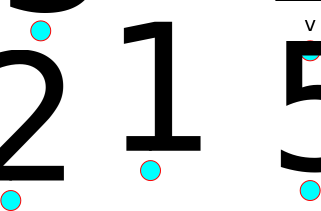
\includegraphics[width=0.8\textwidth]{out/rast_pri_points.eps}
    \caption{Point}
  \end{subfigure}
  \begin{subfigure}[b]{0.3\textwidth}
    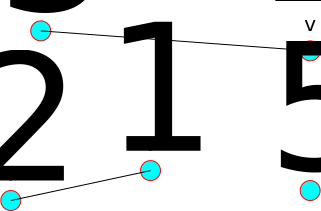
\includegraphics[width=0.8\textwidth]{out/rast_pri_lines.eps}
    \caption{Line}
  \end{subfigure}
  \begin{subfigure}[b]{0.3\textwidth}
    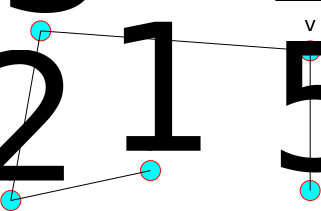
\includegraphics[width=0.8\textwidth]{out/rast_pri_line_strip.eps}
    \caption{Line Strip}
  \end{subfigure}

  \vspace{2em}

  \begin{subfigure}[b]{0.3\textwidth}
    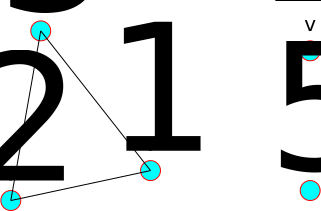
\includegraphics[width=0.8\textwidth]{out/rast_pri_triangle.eps}
    \caption{Triangle}
  \end{subfigure}
  \begin{subfigure}[b]{0.3\textwidth}
    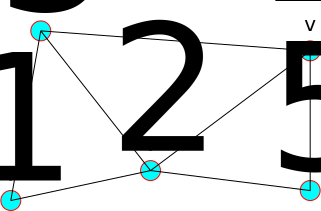
\includegraphics[width=0.8\textwidth]{out/rast_pri_triangle_strip.eps}
    \caption{Triangle Strip}
  \end{subfigure}
  \begin{subfigure}[b]{0.3\textwidth}
    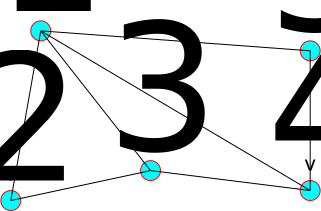
\includegraphics[width=0.8\textwidth]{out/rast_pri_triangle_fan.eps}
    \caption{Triangle Fan}
  \end{subfigure}

  \caption{}
  \label{fig:primitives}
\end{figure}
\FloatBarrier

\subsection{Graphics Pipeline}

\begin{figure}[h!]
  \centering
  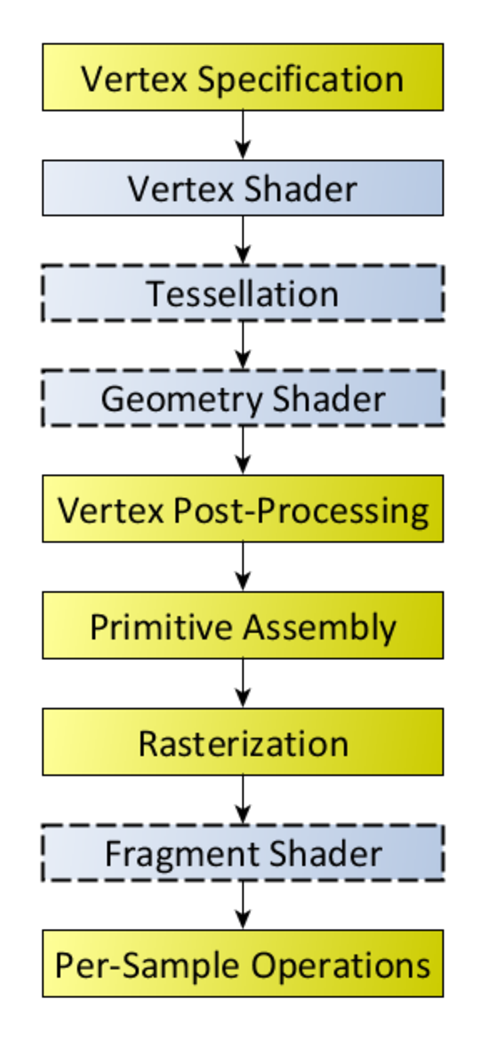
\includegraphics[width=0.25\textwidth]{graphics/rendering_pipeline.eps}
  \caption{OpenGL Pipeline}
  \label{fig:graphics_pipeline}
\end{figure}
\FloatBarrier

\subsection{OpenGL}

Useful (somewhat) OpenGL related stuff to know:

\begin{itemize}
  \item
    Buffers
    \begin{itemize}
      \item
        OpenGL buffers are generated from data in main memory

      \item
        Buffer generation copies data to graphics memory

      \item
        Data in main memory is no longer required

      \item
        OpenGL buffers can be bound to CPU memory addresses to modify buffer
        contents

    \end{itemize}

  \item
    Shaders
    \begin{itemize}
      \item
        Operate per item (per vertex for vertex and tessellation shaders, per
        primitive for geometry shader, per fragment for fragment shader)

      \item
        Data common to all shaders passed as uniforms

    \end{itemize}
\end{itemize}

\section{Transformations}
\label{sec:transformations}

\subsection{Spaces}

\begin{description}
  \item[World] \hfill \\
    3D space containing everything

  \item[Camera] \hfill \\
    3D space containing the view from the camera \\
    Origin is camera position \\
    Obtained through camera transform

  \item[Clip] \hfill \\
    Only the primitives that can be seen by the camera \\
    Obtained through perspective transform

  \item[Normalised Device Coordinates] \hfill \\
    Transformed from clip space \\
    Coordinates normalised to 1 for hardware compatibility

  \item[Viewport Coordinates] \hfill \\
    Coordinates on a particular screen

\end{description}

\subsection{Scale}

Scale matrix to scale by $x$, $y$ and $z$ is each respective axis:
\[
  \left [
    \begin{array}{cccc}
      x & 0 & 0 & 0 \\
      0 & y & 0 & 0 \\
      0 & 0 & z & 0 \\
      0 & 0 & 0 & 1
    \end{array}
  \right ]
\]

\subsection{Translation}

Translation matrix to move by $x$, $y$ and $z$ is each respective axis:
\[
  \left [
    \begin{array}{cccc}
      1 & 0 & 0 & x \\
      0 & 1 & 0 & y \\
      0 & 0 & 1 & z \\
      0 & 0 & 0 & 1
    \end{array}
  \right ]
\]

\subsection{Rotation}

Rotation about $x$ axis by $\theta$:
\[
  \left [
    \begin{array}{cccc}
      1 & 0           & 0         & 0 \\
      0 & cos\theta   & sin\theta & 0 \\
      0 & -sin\theta  & cos\theta & 0 \\
      0 & 0           & 0         & 1
    \end{array}
  \right ]
\]

Rotation about $y$ axis by $\theta$:
\[
  \left [
    \begin{array}{cccc}
      cos\theta   & 0 & sin\theta & 0 \\
      0           & 1 & 0         & 0 \\
      -sin\theta  & 0 & cos\theta & 0 \\
      0           & 0 & 0         & 1
    \end{array}
  \right ]
\]

Rotation about $z$ axis by $\theta$:
\[
  \left [
    \begin{array}{cccc}
      cos\theta   & sin\theta & 0 & 0 \\
      -sin\theta  & cos\theta & 0 & 0 \\
      0           & 0         & 1 & 0 \\
      0           & 0         & 0 & 1
    \end{array}
  \right ]
\]

\subsection{Perspective}

Perspective matrix used to give perspective to camera space.

\begin{figure}[h!]
  \centering
  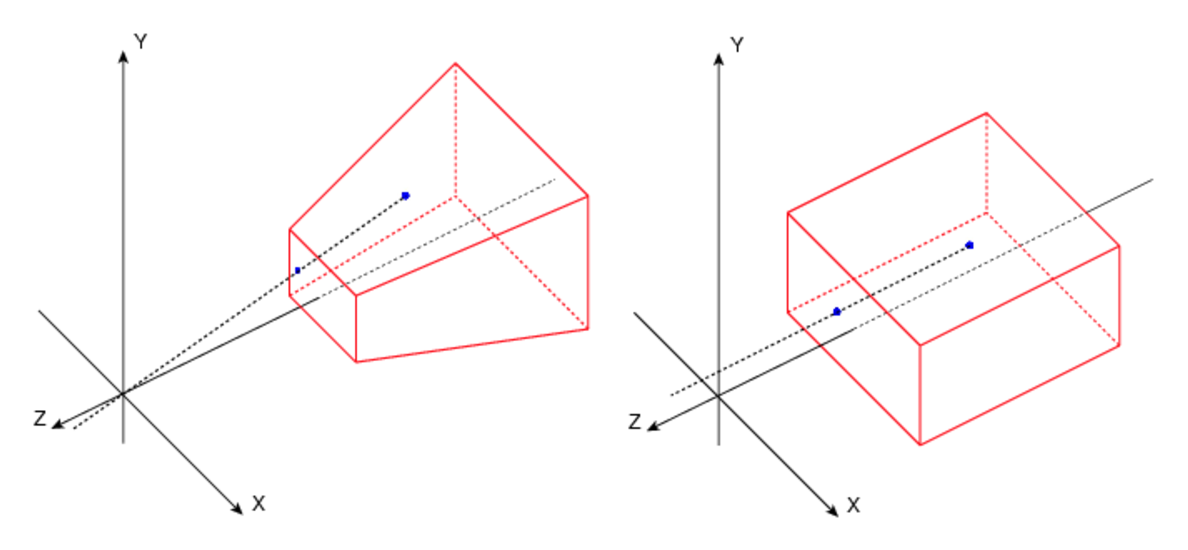
\includegraphics[width=0.6\textwidth]{graphics/perspective-orthographic.eps}
  \caption{Perspective (left) vs Orthographic (right)}
  \label{fig:perspective-orthographic}
\end{figure}
\FloatBarrier

\subsubsection{Orthographic}

Simple clip to a defined box defined by vertices $(left, bottom near)$ and
$(right, top, far)$.
\[
  P =
  \left [
    \begin{array}{cccc}
      \frac{2}{right - left}  & 0                       & 0                     & -\frac{right + left}{right - left} \\
      0                       & \frac{2}{top - bottom}  & 0                     & -\frac{top + bottom}{top - bottom} \\
      0                       & 0                       & \frac{2}{far - near}  & -\frac{far + near}{far - near} \\
      0                       & 0                       & 0                     & 1
    \end{array}
  \right ]
\]

Typically used for "flat" elements, e.g. menu, HUD, etc.

\subsubsection{Perspective}

Traditional perspective as perceived in real life.

\[
  P =
  \left [
    \begin{array}{cccc}
      \frac{f}{aspect}  & 0 & 0                             & 0 \\
      0                 & f & 0                             & 0 \\
      0                 & 0 & \frac{near + far}{near - far} & \frac{2 \cdot near \cdot far}{near - far} \\
      0                 & 0 & -1                            & 0
    \end{array}
  \right ]
\]

where:
\[
  f = \frac{1}{tan(fov / 2)}
\]

and $fov$ is the desired field of view.

\begin{description}
  \item[$x$ and $y$] \hfill \\
    Used to obtain distance along $x$ and $y$ axis with relation to $z$ and
    $fov$

  \item[$z$] \hfill \\
    Scale and translate $z$ position such that $z$ is in the range -1 to 1 after
    division by $w$

  \item[$w$] \hfill \\
    Set to $w = -1 \cdot z = -z$, this is used for the perspective divide

\end{description}

\subsubsection{Perspective Divide}

\url{https://www.khronos.org/opengl/wiki/Vertex_Post-Processing#Perspective_divide}

Have a vector $V$ for a vertex:
\[
  V =
  \left [
    \begin{array}{c}
      V_{x} \\
      V_{y} \\
      V_{z} \\
      w
    \end{array}
  \right ]
\]

Divide components of $V$ by $w$. This operation moves objects that are further
away (in $z$ axis) closer to the centre of the screen, this gives the effect of
a vanishing point.

\subsection{Object definition}

\[
  \left [
    \begin{array}{cccc}
      r_{xx}  & r_{xy}  & r_{xz}  & x \\
      r_{yx}  & r_{yy}  & r_{yz}  & y \\
      r_{zx}  & r_{zy}  & r_{zz}  & z \\
      0       & 0       & 0       & 1
    \end{array}
  \right ]
  \left [
    \begin{array}{c}
      V_{x} \\
      V_{y} \\
      V_{z} \\
      1
    \end{array}
  \right ]
\]

$(x, y, z)$ is the object position.

$r$ is the object orientation.

$(r_{xx}, r_{xy}, r_{xz})$ is the object left vector.

$(r_{yx}, r_{yy}, r_{yz})$ is the object up vector.

$(r_{zx}, r_{zy}, r_{zz})$ is the object facing vector.

The vertices of the object $V$ are transformed using the object matrix.

\subsection{MVP matrix}

Three stages of the standard transformation pipeline:

\begin{description}
  \item[Model] \hfill \\
    Local space to the world space

  \item[View] \hfill \\
    World space to camera space

  \item[Projection] \hfill \\
    Camera space to clip space

\end{description}

\section{Vertex/Geometry Operation}

\subsection{Amplification (Tessellation Shader)}

\url{https://www.khronos.org/opengl/wiki/Tessellation}

\begin{itemize}
  \item
    Tessellator runs after vertex shader

  \item
    Operates on patch primitives (generic $n$-sided primitive)

  \item
    Outputs tessellated geometry in either: triangles, quads or isolines

  \item
    Tessellation Control Shader is used to set tessellation level and perform
    any required patch transformations

    (Tessellation Control Shader is optional)

  \item
    Tessellation Evaluation Shader takes abstract coordinates generated by the
    tessellator and the patch coordinates and calculates the vertices of the
    output geometry

    (Tessellation Evaluation Shader is mandatory)

  \item
    Level of tessellation is set for inner and outer regions of tessellated
    geometry

    \begin{itemize}
      \item
        Inner level controls tessellation inside the area

      \item
        Outer level controls tessellation outside the area

      \item
        Edges that are shared between two tessellated areas must share the same
        outer tessellation level and vertex calculation to ensure continuity
        between areas
    \end{itemize}

\end{itemize}

\begin{figure}[h]
  \centering

  \begin{subfigure}[b]{0.3\textwidth}
    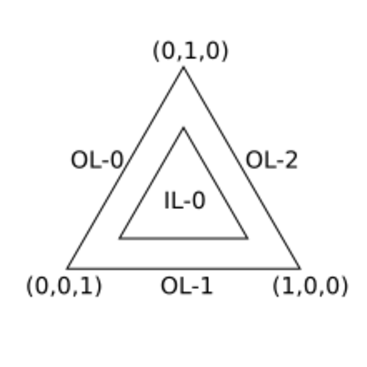
\includegraphics[width=0.8\textwidth]{graphics/tess_triangle.eps}
    \caption{Triangle}
  \end{subfigure}
  \begin{subfigure}[b]{0.3\textwidth}
    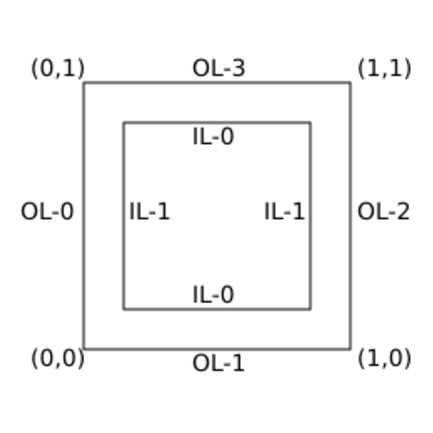
\includegraphics[width=0.8\textwidth]{graphics/tess_quad.eps}
    \caption{Quad}
  \end{subfigure}
  \begin{subfigure}[b]{0.3\textwidth}
    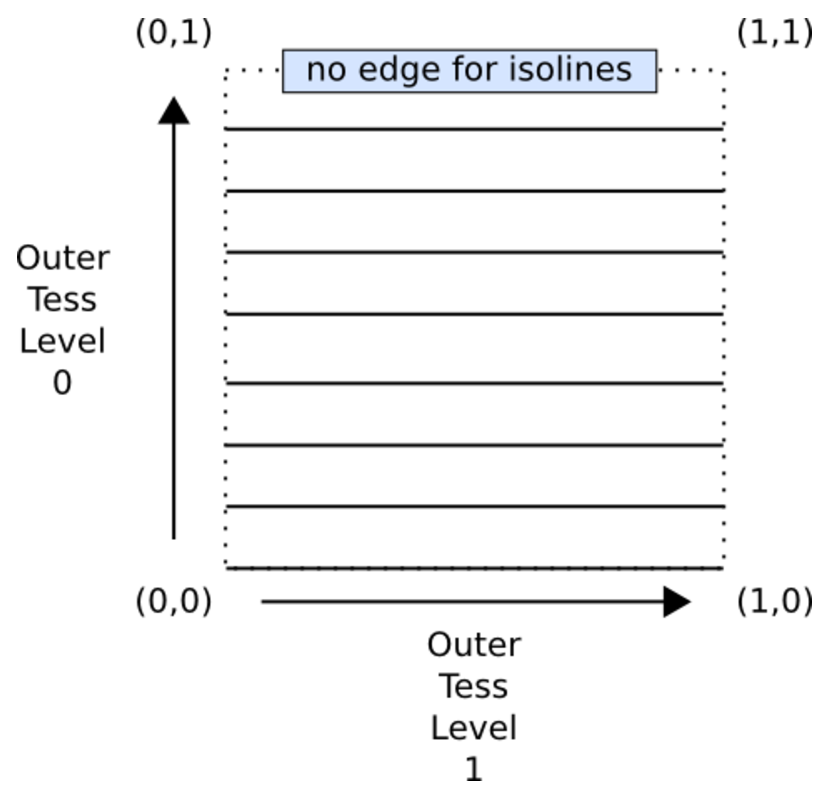
\includegraphics[width=0.8\textwidth]{graphics/tess_isoline.eps}
    \caption{Isoline}
  \end{subfigure}

  \caption{Tessellation levels}
  \label{fig:tess_levels}
\end{figure}
\FloatBarrier

\subsection{Generation (Geometry Shader)}

\url{https://www.khronos.org/opengl/wiki/Geometry_Shader}

\begin{itemize}
  \item
    Geometry shader runs after tessellator

  \item
    Takes single primitive as input and outputs zero or more new primitives
    (limited types of primitives supported: points, lines \& triangles)

  \item
    Used to generate new (additional) geometry based on (limited) existing
    geometry

  \item
    e.g. basic graphical particle system in which points are sent to the GPU
    pipeline and are converted into quads by the geometry shader

    This saves (~75\%) CPU time copying primitives to the GPU

\end{itemize}

\subsection{Clipping}

\url{https://www.khronos.org/opengl/wiki/Vertex_Post-Processing#Clipping}

\begin{itemize}
  \item
    Remove geometry outside of viewing volume, reduced GPU load in rasterising
    (parts of) primitives that will never be seen

  \item
    Whole primitives that are outside viewing volume are simply culled as a
    whole

  \item
    Primitives that are partially outside are split at the boundary of the
    viewing volume and new primitives are created as needed to fill any space
    created inside the viewing volume (e.g. in the case of triangle clipping)

\end{itemize}

\subsection{Face Culling}

\url{https://www.khronos.org/opengl/wiki/Face_Culling}

\begin{itemize}
  \item
    Removes (culls) faces that will not be seen due to facing away from the
    camera

  \item
    Can cull front, back or all faces

    Culling all faces effectively disables the rasteriser for triangle based
    primitives

  \item
    Front and back faces are determined by the winding order of the vertices of
    triangles

\end{itemize}

\section{Fragment Operations}
\label{sec:fragment_operations}

\url{https://www.khronos.org/opengl/wiki/Per-Sample_Processing}

\subsection{Interpolation}

\Para{Lines}

Colour at point $p$ computed through simple linear interpolation between
vertices $v_{0}$ and $v_{1}$.
\begin{align*}
  C_{p} &= (C_{b} * t) + (C_{a} * (1 - t)) \\
  t &= |(v_{1} - p) / (v_{1} - v_{0})|
\end{align*}

\Para{Triangles}

Use Barycentric coordinates (section \ref{sec:barycentric}).
\[
  C_{p} = (\alpha * C_{a}) + (\beta * C_{b}) + (\gamma * C_{c})
\]

\subsection{Scissor testing}

\url{https://www.khronos.org/opengl/wiki/Scissor_Test}

\begin{itemize}
  \item
    Fragments outside of a given rectangle on the screen are discarded

  \item
    Can set unique scissor box per viewport
\end{itemize}

\subsection{Stencil testing}

\url{https://www.khronos.org/opengl/wiki/Stencil_Test}

\begin{itemize}
  \item
    Uses additional buffer attached to active framebuffer

  \item
    Each fragment has a stencil value

  \item
    Stencil value of a given fragment is tested against value in stencil buffer,
    if the test passes the fragment is used

  \item
    Operation on stencil buffer can be configured based on the result of the
    stencil and depth tests: keep current value, set to zero, invert current
    value, replace current value, increment, decrement, increment with wrap,
    decrement with wrap.

  \item
    Test is configurable: always, never, $=$, $\neq$, $<$, $\leq$, $>$, $\geq$

  \item
    Initial fragment stencil value is given for all fragments when configuring
    the stencil test

  \item
    Stencil testing can be performed on either front or back faces of a
    primitive, or both (state is held for both faces)

\end{itemize}

\subsection{Depth Buffer / Depth Test}

\url{https://www.khronos.org/opengl/wiki/Depth_Test}

Have a depth buffer which records the depth ($z$ coordinate) of the fragment
that has been rendered on a each pixel.

\begin{enumerate}
  \item[1]
    When a pixel is to be shaded compare the $z$ coordinate of the new fragment
    with that in the depth buffer $D_{i}$

  \item[2.1]
    If $x \leq D_{i}$ then depth test passes, the pixel is shaded based on the
    new fragment and the depth buffer updated

  \item[2.1]
    Otherwise the test fails and the fragment is discarded

  \item[3]
    The depth buffer is rest to maximum depth at the start of each frame

\end{enumerate}

Can have "z fighting" when two objects with close $z$ coordinates are rasterised
inside each other. A higher precision depth buffer avoids this.

\subsection{Blending}

\url{https://www.khronos.org/opengl/wiki/Blending}

Transparency denoted by alpha value in colour.

$\alpha = 1$ denotes full opacity, $\alpha = 0$ denotes full transparency.

Colour computed by blend equation:
\[
  C = (C_{source} * F_{source}) + (C_{dest} * F_{dest})
\]

Factors $F_{source}$ and $F_{dest}$ are usually programmable but a common
approach is standard linear blending:
\begin{align*}
  F_{source} &= \alpha \\
  F_{dest} &= 1 - \alpha
\end{align*}

One other alternative is additive blending:
\begin{align*}
  F_{source} &= 1 \\
  F_{dest} &= 1
\end{align*}

\section{Texture Mapping}

\begin{itemize}
  \item
    Texture coordinates $(u, v)$ defined per vertex

  \item
    Coordinated interpolated to obtain per fragment texture coordinates

  \item
    $(u, v)$ are normalised texture coordinates within $[0, 1]$

  \item
    Textures coordinates out of the $[0, 1]$ can be handled differently:

    \begin{description}
      \item[Clamp] \hfill \\
        Anything above 1 is set to 1 \\
        Anything below 0 is set to 0

      \item[Repeat] \hfill \\
        $1.1 = 0.1$ \\
        $-0.1 = 0.9$ \\
        etc.

      \item[Mirror] \hfill \\
        $1.1 = 0.9$ \\
        $-0.1 = 0.1$ \\
        etc.

    \end{description}

  \item
    All textures for a mesh typically stored in a single texture image

\end{itemize}

\subsection{Affine Transform}

Textures may not appear correctly if an object is tilted with respect to the
camera.

Caused by texture interpolation being linear but not fragment area.

Solution is to use affine transform:

\begin{enumerate}
  \item[1]
    Divide texture coordinates by $P_{w}$

  \item[2]
    Interpolate texture coordinates

  \item[3]
    Multiply by $P_{w}$

\end{enumerate}

\subsection{Bilinear Filtering}

\begin{itemize}
  \item
    When a texture is viewed close enough to the camera such that the rasterised
    object takes up more pixel space than the texture image

  \item
    Sample multiple texels and blend them together

    e.g. for texel coordinate 7.6 blend colour of texel 7 and 8 by factor 0.6

\end{itemize}

\subsection{MIP mapping /  minification}

\begin{itemize}
  \item
    Generating smaller textures using the original fill size texture so that
    objects further away can sample a smaller texture

  \item
    Forms a set of textures in decrecing size, known as a MIP chain

  \item
    MIP map is selected using the level of detail (LOD) $\lambda$

  \item
    This is calculated using the derivatives of the interpolated $x$ and $y$
    texture coordinates, i.e. how fast the texture coordinates are changing

  \item
    Faster change in texture coordinates (higher $\lambda$) means less unique
    texels hence less detail. The size of $\lambda$ denotes how far down the MIP
    change the texture is selected

  \item
    MIP chain is pre processed when the texture is loaded

  \item
    Requires more memory to store entire MIP chain opposed to a single texture,
    but gives faster processing as less work needs to be done during
    rasterisation and gives a better texture quality due to texel averaging

\end{itemize}

\subsubsection{Trilinear filtering}

\begin{itemize}
  \item
    Similar to bilinear filtering (operating in $x$ and $y$ axes) but also
    operating in $z$ axis to interpolate between two MIP map levels

  \item
    Solves issue when an object spans multiple MIP levels and a noticeable line
    where the texture quality changes can be seen

\end{itemize}

\section{Scene Hierarchy and Skeletal animation}

\subsection{Scene Graphs}

\begin{itemize}
  \item
    Hierarchical tree structure of meshes

  \item
    Each mesh has a model matrix that gets applied to it and all its children

  \item
    Typically use a tree as shallow as possible to reduce traversal time

  \item
    Can include many other (non graphical) objects on the tree:

    \begin{itemize}
      \item Sound emitters
      \item Shaders
      \item etc.
    \end{itemize}

\end{itemize}

Need to ensure transparent objects are drawn in the correct order. Solution is
to add a "transparency" tag to each node.

When processing objects:

\begin{enumerate}
  \item[1]
    Traverse the tree and build a list of opaque objects and a list of
    transparent objects

  \item[2]
    Render all the opaque objects

  \item[3]
    Sort the list of transparent objects by their $z$ position

  \item[4]
    Render transparent object from furthest away to closest

\end{enumerate}

\subsection{Animation}

\begin{itemize}
  \item
    Can do simple animation by manipulating a tree of objects and their model
    matrices

    This works well for simple objects such as cars and robots

  \item
    It will not work for objects that have a flexible skin (such as humans)

\end{itemize}

\subsubsection{Skinned meshes}

\begin{itemize}
  \item
    Model has internal skeleton made up of several joints which can be
    positioned and rotated relative to each other

  \item
    Use a mesh (skin) for a subsection of (or entire) skeleton and set position
    of vertices on the mesh using weightings based on joint positions

  \item
    Two variants:

    \begin{itemize}
      \item
        Each skin vertex has a position and a set of joints it is influenced by

      \item
        Each vertex is relative to a number of anchors

        Each anchor has a position and a joint it is relative to

    \end{itemize}

\end{itemize}

\section{Lighting}

\subsection{Normals}

\begin{itemize}
  \item
    Unit vector perpendicular to the surface

  \item
    Can be calculated using cross product of two side vectors

  \item
    Usually stored as part of the model

  \item
    Vertex normals are interpolated across the primitive

  \item
    Interpolation may cause problems if an object has sharp corners

  \item
    Cannot simply transform normals

    Can use model matrix to transform is scale is uniform

\end{itemize}

\subsection{Lighting Models}

\begin{description}
  \item[Static lighting] \hfill \\
    Combining texture with a light map. \\
    No real time updates. \\
    No additional computation.

  \item[Flat shading] \hfill \\
    Per surface lighting. \\
    Single value used on a surface. \\
    Computationally fast.

  \item[Gourard shading] \hfill \\
    Per vertex shading. \\
    Interpolated across primitive. \\
    More computationally expensive.

  \item[Phong shading] \hfill \\
    Per fragment lighting. \\
    Most computationally intensive.

\end{description}

\subsection{Phong Reflection Model}

Types of light:

\begin{description}
  \item[Ambient] \hfill \\
    Lights all faces of all objects in a scene equally

  \item[Diffuse] \hfill \\
    Light from a source that has been scattered evenly

  \item[Specular] \hfill \\
    Light from a source that has been reflected towards the camera

\end{description}

Lighting colour $c$ of a fragment (for a single light):
\begin{align*}
  c &= c_{a} + (c_{d} + c_{s}) \times a \\
  c_{d} &= (N \cdot |(L - P)|) \times C_{d} \\
  c_{s} &= (N \cdot \frac{1}{2}(V + L))^{n} \times C_{s}\\
  a &= 1 - \frac{L}{L_{max}}
\end{align*}

where:

\begin{itemize}
  \item
    $k_{a}$ is the constant ambient light for the scene

  \item
    $L_{max}$ is the maximum distance that a light source can be away from a
    source

  \item
    $L$ is the distance from the light source to the surface

  \item
    $n$ is the specular power (higher for shinier materials)

  \item
    $C_{d}$ and $C_{s}$ are colours of the diffuse and specular light

  \item
    $P$ is the fragment position

  \item
    $V$ is the view vector

  \item
    $L$ is the light vector

  \item
    $N$ is the normal

\end{itemize}

Normal $N$ can be calculated using two side vectors: $N = (v_{0} - v_{1}) \times
(v_{0} - v_{2})$

Attenuation factor $a$ ensures that the light gets weaker as the light source
moves away from the surface.

\subsection{Bump mapping}

\begin{itemize}
  \item
    Adds additional surface texture/bump detail to Phong lighting model

  \item
    Surface texture stored in bump map (texture) in tangent space

    Must be transformed to world space before used in lighting calculations

  \item
    Perform translation using binormal (see figure \ref{fig:binormal_calc})

    $B = cross(N, T)$

  \item
    Transformation is performed using tangent binormal normal matrix

    \[
      \left [
        \begin{array}{ccc}
          T_{x} & B_{x} & N_{x} \\
          T_{y} & B_{y} & N_{y} \\
          T_{z} & B_{z} & N_{z}
        \end{array}
      \right ]
    \]

    $N_{w} = TBN \cdot N$

\end{itemize}

\begin{figure}[h!]
  \centering
  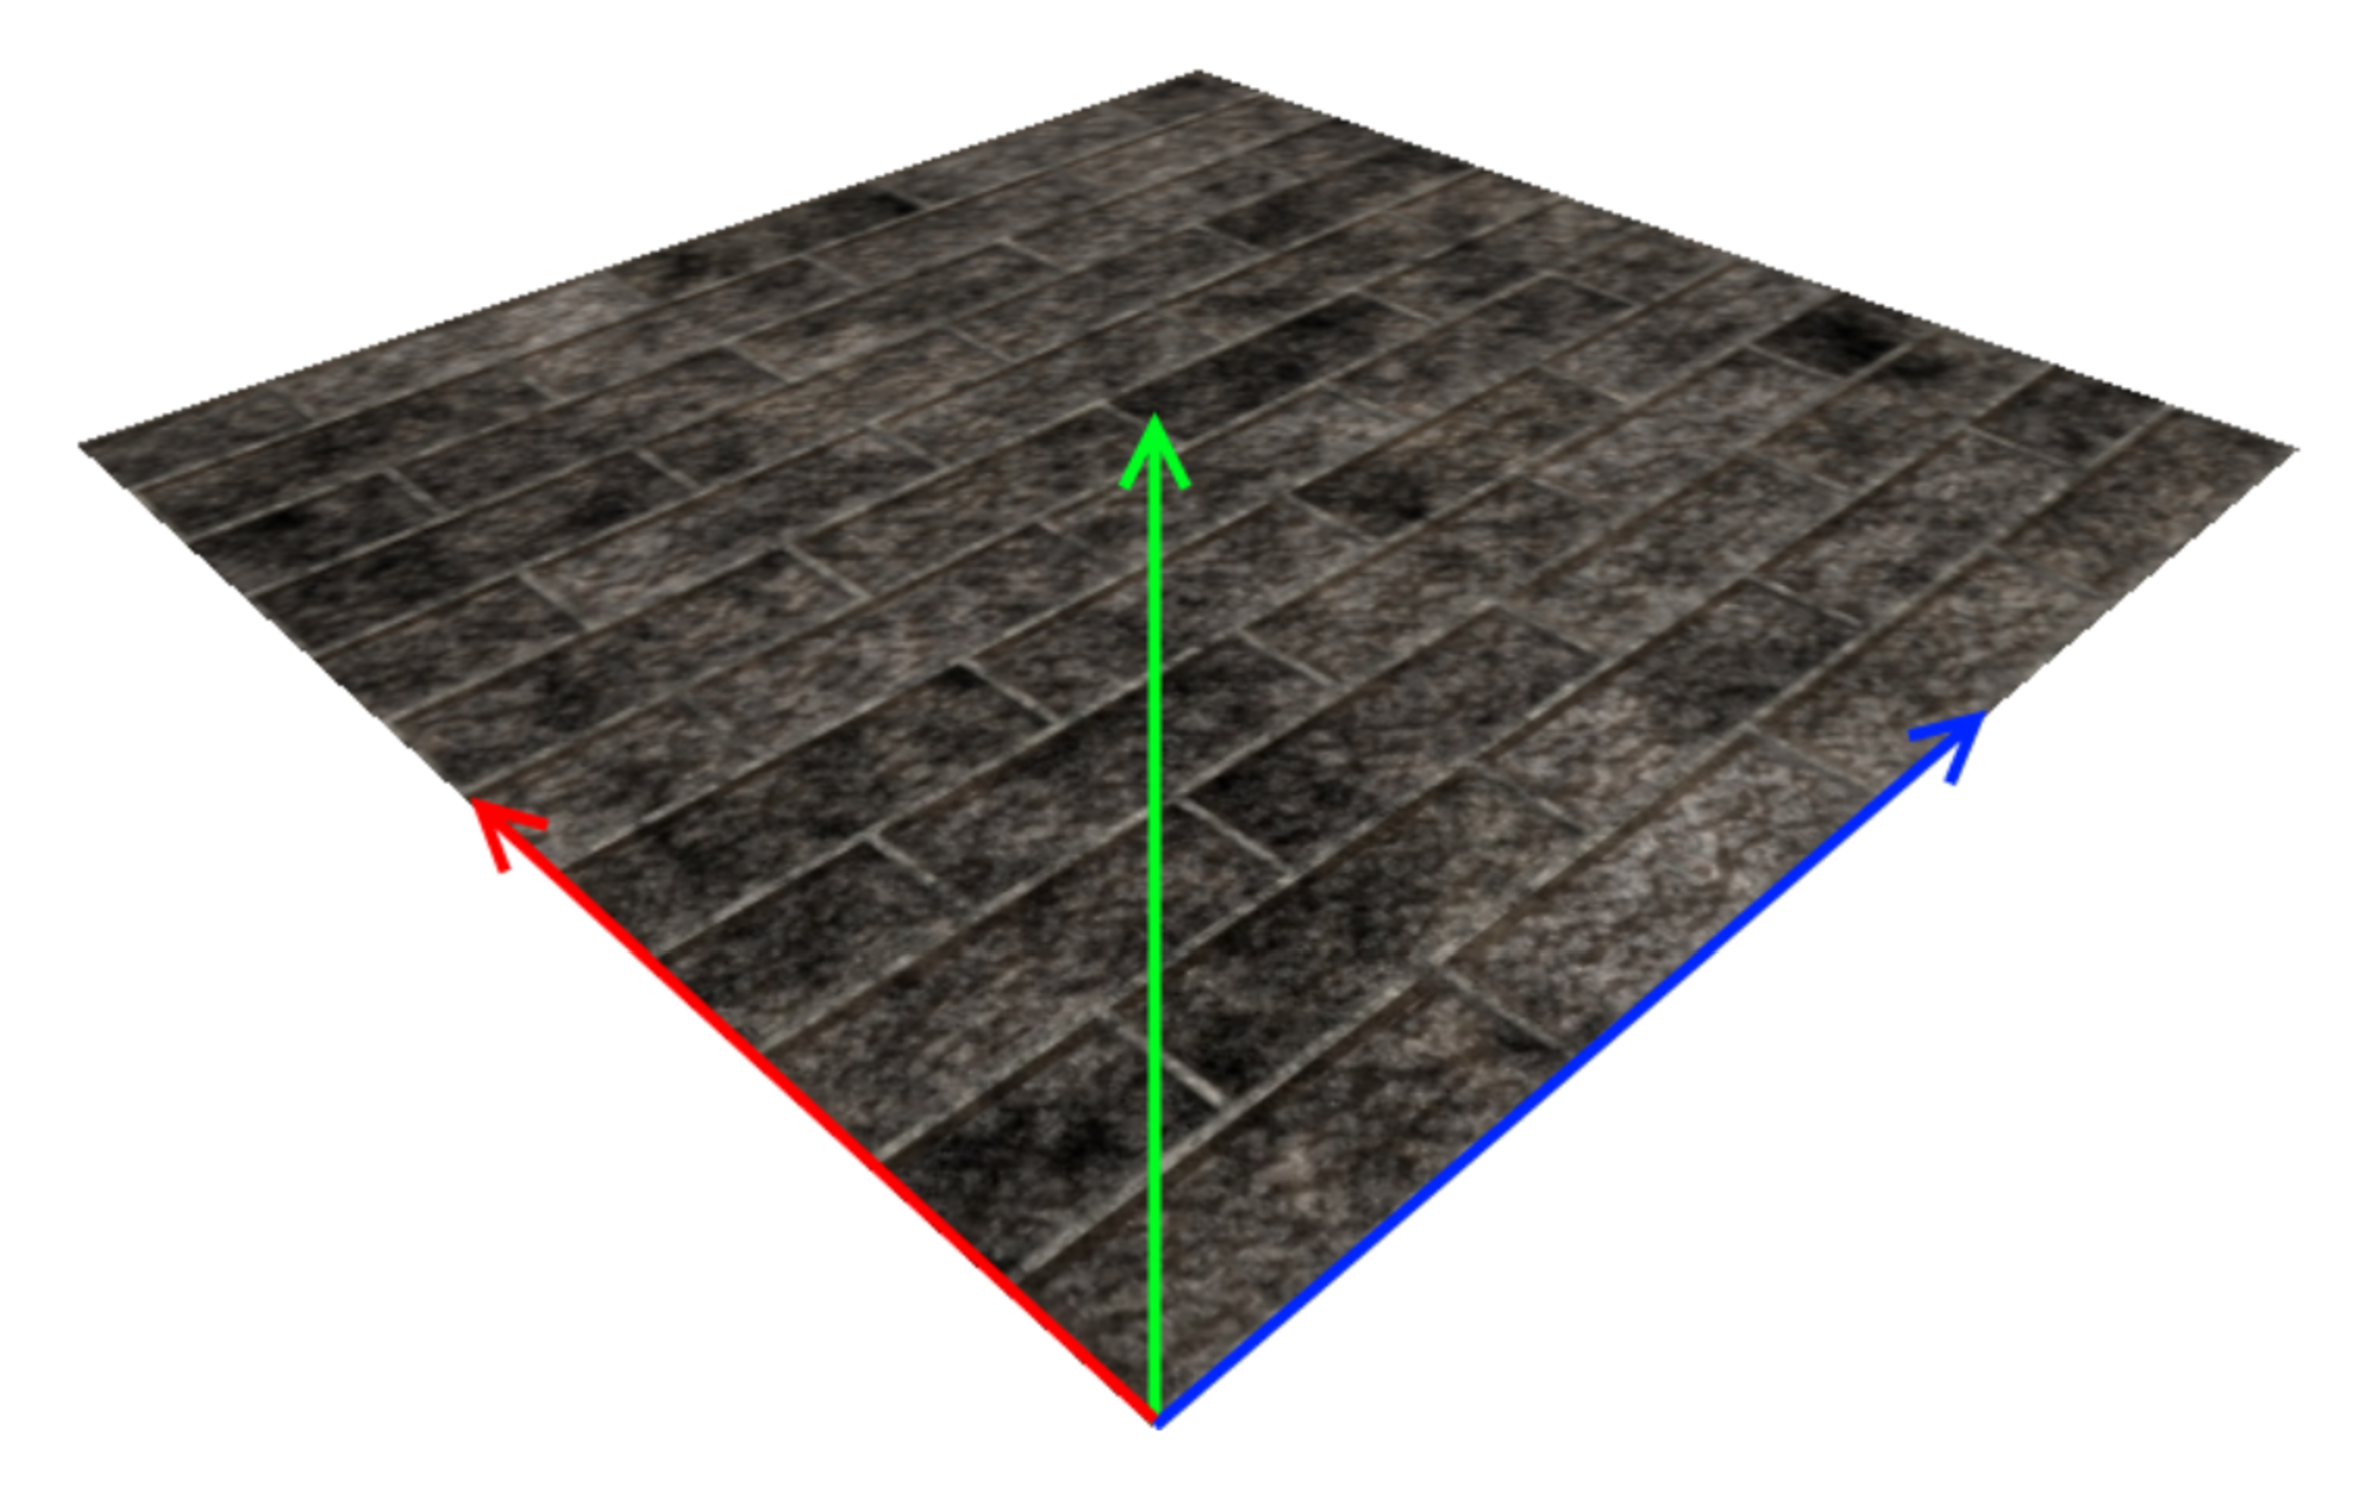
\includegraphics[width=0.4\textwidth]{graphics/binormal_calc.eps}
  \caption{Binormal calculation \\
           Green = Normal, Blue = Tangent, Red = Binormal}
  \label{fig:binormal_calc}
\end{figure}
\FloatBarrier

\subsection{Shadow mapping}

\begin{itemize}
  \item
    First pass

    \begin{itemize}
      \item
        Obtain a shadow map for each light that can cast a shadow.

        1 map for unidirectional lights, 6 maps for omnidirectional lights.

      \item
        Maps are generated by rendering the scene from the position of the light
        in the relevant direction.

        The map is the depth buffer.

      \end{itemize}

    \item
      Second pass

      \begin{itemize}
        \item
          Scene rendered from point of view of camera

        \item
          Shadow matrix is passed to shaders, this is the MVP matrix used for
          light map in first pass

        \item
          Shadow map used to determine position of each fragment from
          perspective of the light

        \item
          In fragment shader compare the $z$ component of the fragment to the
          value from the shadow buffer.

          If $z \leq light \: depth$ then the fragment is in front of the
          closest object in the shadow map, therefore is lit by the light.a

          if $z > light \: depth$ then the fragment is behind the nearest object
          to the light so is in shadow.

      \end{itemize}

    \item
      Shadow map sampling

      \begin{itemize}
        \item
          Shadow map is sampled similar to other textures, however a specialised
          sampler is used that takes a 4 component vector and returns the result
          of the shadow depth test

        \item
          A bias matrix (uniform scale by 0.5, uniform translation by 0.5) is
          used to convert from clip space coordinates (-1 to 1) to texture
          coordinates (0 to 1)

      \end{itemize}

\end{itemize}

\subsubsection{Issues}

\begin{description}
  \item[Surface Acne] \hfill \\

    \begin{itemize}
      \item
        Depth buffer is not high accuracy, especially for objects far from the
        camera position (or objects far from the light in a shadow map)

      \item
        Can cause issues when occluding objects and the surface they occlude are
        both visible by the camera

      \item
        In this case additional shadows may be rendered due to error in the
        depth values of the occluding and visible surfaces

      \item
        One solution is to offset the vertices used in the shadow map depth
        comparison, either towards the camera or along their normal

        This increases the difference between the two values and reduced the
        likelihood of error accumulation affecting the result of the shadow
        depth test

    \end{itemize}

  \item[Aliasing] \hfill \\

    \begin{itemize}
      \item
        Low resolution of depth buffer for far geometry can cause poor
        resolution shadows

      \item
        Area of geometry far from camera/light is "covered" by fewer samples
        than the same sized area near to the camera/light

      \item
        Commonly an issue when an object is far from a light but close to the
        camera

      \item
        Simplest solution is to increase resolution of shadow map

    \end{itemize}

\end{description}

\subsection{Deferred Rendering}

\begin{itemize}
  \item
    In the conventional approach to lighting every fragment is processed by the
    lighting calculation even if they are not visible in the scene

    When many lights are present in the scene this can add up to a considerable
    amount of processing overhead processing fragments that have no influence on
    the final rendered scene

    This is the same with objects that are not in range of a given light

  \item
    Deferred rendering allows lighting calculations to be run in image space
    (the final rendered image), this means that only fragments that are visible
    in the final rendered scene will have lighting calculations applied to them

  \item
    Requires splitting data up into several screen sized buffers containing
    information used in lighting calculations

    This is known as the G-buffer

    Possible contents:
    \begin{itemize}
      \item
        Diffuse colours

      \item
        Normals

      \item
        Depth

      \item
        Specular intensity

      \item
        Post processing flags

      \item
        (any per fragment data)

    \end{itemize}

  \item
    Lighting calculations are only performed within the volume of a given light,
    removes calculations for fragments that are outside of a given lights reach

  \item
    In the second pass it is already known what fragments are in the final image
    (from the G-buffer) therefore no calculations take place for fragments that
    do not contribute to the final image

  \item
    Video memory and bandwidth can be an issue due to the large amount of space
    taken by the G-buffer

  \item
    Still does not help with issue of lighting transparent objects

  \item
    May need to perform anti-aliasing on final scene to remove jaggedness from
    edges

\end{itemize}

\subsubsection{Light volumes}

\begin{itemize}
  \item
    In second pass volumes are rendered for each light

  \item
    Light volume encapsulates area which is lit by the light

  \item
    For example, for a simple point light the volume is simple a sphere, for a
    spotlight it could be a cone

  \item
    In view space a light volume could encapsulate an object that is in reality
    far away from the light

    For this reason depth testing in the third stage must be performed

\end{itemize}

\subsubsection{Workflow}

\begin{enumerate}
  \item[1]
    Fill G-Buffer

    \begin{itemize}
      \item
        Very similar to conventional rendering process

      \item
        Transform vertex positions by MVP matrix

      \item
        Sample diffuse colour from texture

      \item
        Fill relevant data in G-buffer

    \end{itemize}

  \item[2]
    Lighting Calculations

    \begin{itemize}
      \item
        Render light volumes into scene, marking fragments that may be affected
        by lights

      \item
        In fragment shader the world position of the fragment is reconstructed
        using the depth map from the G-buffer

        Can then determine if lighting calculation should be performed or if the
        fragment should be discarded (if outside light volume)

      \item
        Additive blending is used to combine contributions from multiple lights

    \end{itemize}

  \item[3]
    Generate Final Image

    \begin{itemize}
      \item
        Draw a screen sized quad

      \item
        Texture using blend of lighting attachment textures and diffuse texture
        (from G-buffer)

    \end{itemize}

\end{enumerate}

\section{Post processing}

\begin{itemize}
  \item
    Scene is rendered into a framebuffer to allow post processing stages to
    manipulate the rendered scene as a texture

  \item
    Textures are bound to framebuffers as attachments that can contain colour,
    depth and stencil data

  \item
    Once scene has been rendered into framebuffer the attachments can be
    manipulated in further pipeline stages as regular textures

  \item
    Textures used as framebuffer attachments cannot be compressed
    (compression/decompression overhead would be undesirable anyway) but can be
    packed (e.g. using a single texture for depth and stencil attachments)

  \item
    A  processing stage renders a single quad that fills the screen which is
    then textured using the colour attachment texture from the framebuffer the
    scene was rendered into

  \item
    Processing stages may be cascaded using multiple processing render passes
    into multiple framebuffers

    An alternative to this is "ping-pong" texturing, in which a single
    framebuffer and two textures are used and each processing stage samples from
    one texture and buffers to the other alternately

  \item
    As the scene render pass is available as a texture effects that depend on
    multiple fragments (e.g. blur) are now possible

    Such effects are not possible without this post processing stage as in the
    standard pipeline the fragment shader does not have access to adjacent (or
    any) fragments other than the one it is operating on

\end{itemize}

\end{document}
